\documentclass[12pt,utf8,notheorems]{beamer}

\usepackage[ngerman]{babel}

\usepackage{amsmath,amssymb}
%\usepackage[framed,amsmath,thmmarks,hyperref]{ntheorem}

%\usepackage[small,nohug]{diagrams}
%\diagramstyle[labelstyle=\scriptstyle]

%\usepackage[protrusion=true,expansion=false]{microtype}

%\usepackage{lmodern}
\usepackage{nicefrac}
\usepackage{tabto}
\usepackage{tikz}
\usetikzlibrary{decorations.pathreplacing}
\usepackage{bussproofs}
\usepackage{stmaryrd}

%\usepackage[natbib=true,style=numeric]{biblatex}
%\usepackage[babel]{csquotes}
%\bibliography{lit}

%\usepackage{hyperref}

\setlength\parskip{\medskipamount}
\setlength\parindent{0pt}

%\theoremseparator{:}
\theoremstyle{plain}  %nonumberplain
%\newtheorem{beh}{Behauptung}
\newtheorem{proposition}{Proposition}
\newtheorem{corollary}{Korollar}
\newtheorem{theorem}{Satz}
\theoremstyle{definition}
\newtheorem{definition}{Definition}
%\newtheorem{kor}{Korollar}
%\newtheorem{satz}{Satz}
%\newtheorem{lemma}{Lemma}
%\newtheorem{hilfsaussage}{Hilfsaussage}
%\theorembodyfont{\normalfont}
\newtheorem{axiom}{Axiom}
%\newtheorem{defnprop}{Definition/Proposition}
%\newtheorem{bem}{Bemerkung}
%\newtheorem{bsp}{Beispiel}
%\theoremsymbol{\ensuremath{\openbox}}
%\newtheorem{proof}{Beweis}
%\newtheorem{defn}{Definition}

\newcommand{\lra}{\longrightarrow}
\newcommand{\lhra}{\ensuremath{\lhook\joinrel\relbar\joinrel\rightarrow}}
\newcommand{\thlra}{\relbar\joinrel\twoheadrightarrow}

\newcommand{\Z}{\mathbb{Z}}
\renewcommand{\C}{\mathbb{C}}
\newcommand{\N}{\mathbb{N}}
\newcommand{\Hom}{\mathrm{Hom}}
\newcommand{\Spur}[1]{\operatorname{Spur}#1}
\newcommand{\SpurDyn}[1]{\operatorname{Spur}\left(#1\right)}
\newcommand{\rank}[1]{\operatorname{rank}#1}
\newcommand{\Ker}[1]{\operatorname{ker}#1}
\newcommand{\Bild}[1]{\operatorname{im}#1}
\newcommand{\sgn}[1]{\operatorname{sgn}#1}
\newcommand{\id}{\mathrm{id}}
\newcommand{\Aut}[1]{\operatorname{Aut}(#1)}
\newcommand{\GL}[1]{\operatorname{GL}(#1)}
\newcommand{\freist}{\_{}\_{}}

\renewcommand{\O}{\mathcal{O}}
\renewcommand{\P}{\mathcal{P}}
\newcommand{\1}{\mathbf{1}}
\renewcommand{\_}{\mathpunct{.}\,}
\newcommand{\?}{\,{:}\,}
\newcommand{\seq}[1]{\mathrel{\vdash\!\!\!_{#1}}}
\renewcommand{\ll}[1]{\llbracket{#1}\rrbracket}

\newcommand{\XXX}[1]{\textcolor{red}{#1}}

%\newarrow{Equals}=====

\title{Intuitionistische Logik}
\author{Ingo Blechschmidt \\ mit Illustrationen von Carina Willbold}
%\subtitle{Vektorbündel, K-Theorie und \\ charakteristische Klassen}
\institute{Sommerakademie in Neubeuern}
\date{7. August 2012}

%\usetheme{Warsaw}  %Warsaw, Berkeley?
\usetheme{Warsaw}
\useoutertheme{split}
\usecolortheme{seahorse}
\usefonttheme{serif}
\usepackage{palatino}
\useinnertheme{rectangles}
%\usepackage{bookman}
%\setbeamercovered{transparent}

\setbeamertemplate{navigation symbols}{}
\setbeamertemplate{footline}{}
\setbeamertemplate{headline}{}

\beamertemplateboldcenterframetitle
%\setbeamerfont{frametitle}{size={\Large}}

\newenvironment{changemargin}[2]{%
  \begin{list}{}{%
    \setlength{\topsep}{0pt}%
    \setlength{\leftmargin}{#1}%
    \setlength{\rightmargin}{#2}%
    \setlength{\listparindent}{\parindent}%
    \setlength{\itemindent}{\parindent}%
    \setlength{\parsep}{\parskip}%
  }%
  \item[]}{\end{list}}

\begin{document}

\setbeameroption{show notes}
\setbeamertemplate{note page}[plain]

\frame[plain]{
  \begin{center}
    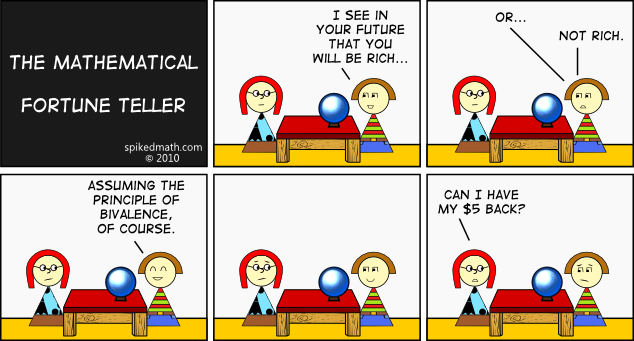
\includegraphics[scale=0.65]{fortune-teller.png}
  \end{center}
}

\frame{\titlepage}
\frame[t]{\frametitle{Gliederung}\begin{minipage}{\textwidth}\begin{small}\tableofcontents\end{small}\end{minipage}}

\section{Einführung}

\subsection{Informale Bedeutung logischer Formeln}
\frame[t]{\frametitle{Informale Bedeutung logischer Formeln}
  \tikz[remember picture] \node[coordinate,yshift=0.0em] (n0) {};
  \vspace{-1.5em}
  \begin{description}\small
    \item[$\bot$] Es stimmt eine Falschheit.
    \tikz[remember picture] \node[coordinate,yshift=0.5em] (n2) {};
    \item[$A \wedge B$] $A$ und $B$ stimmen.
    \item[$A \vee B$] $A$ oder $B$ stimmt.
    \item[$A \Rightarrow B$] Sollte~$A$ stimmen, dann auch~$B$.
    \item[$\forall x{:}X\_\! A(x)$] Für alle~$x\?X$ stimmt jeweils~$A(x).$
    \item[$\exists x{:}X\_\! A(x)$] Es gibt mindestens ein~$x\?X$, für das~$A(x)$
    stimmt.
    \tikz[remember picture] \node[coordinate,yshift=-0.0em] (n1) {};
  \end{description}
  \vspace{1em}

  \begin{description}\small
    \item[$\bot$] 
    \tikz[remember picture] \node[coordinate,yshift=0.5em] (n5) {};%
    Wir haben Beleg für eine Falschheit.
    \item[$A \wedge B$] Wir haben Beleg für~$A$ und für~$B$.
    \item[$A \vee B$] Wir haben Beleg für~$A$ oder für~$B$.
    \item[$A \Rightarrow B$] Sollten wir Beleg für~$A$ haben, können wir
    (gleichmäßig) auch Beleg für~$B$ konstruieren.
    \item[$\forall x{:}X\_\! A(x)$] Wir können (gleichmäßig) für alle~$x\?X$
    Belege für~$A(x)$ konstruieren.
    \item[$\exists x{:}X\_\! A(x)$] Wir haben ein~$x\?X$ zusammen mit Beleg
    für~$A(x)$.
    \tikz[remember picture] \node[coordinate,yshift=-0.0em] (n4) {};
  \end{description}

  \begin{tikzpicture}[overlay,remember picture]
    \path (n2) -| node[coordinate] (n3) {} (n0);
    \path (n1) -| node[coordinate] (n33) {} (n0);
    \draw[thick,decorate,decoration={brace,amplitude=5pt}]
            (n33) -- (n3) node[midway,left=4pt] {kl.};
    \path (n5) -| node[coordinate] (n6) {} (n0);
    \path (n4) -| node[coordinate] (n44) {} (n0);
    \draw[thick,decorate,decoration={brace,amplitude=5pt}]
            (n44) -- (n6) node[midway,left=4pt] {int.};
  \end{tikzpicture}

  \begin{tikzpicture}[remember picture,overlay]  
    \node [xshift=-1cm,yshift=-6cm] at (current page.north east)
      {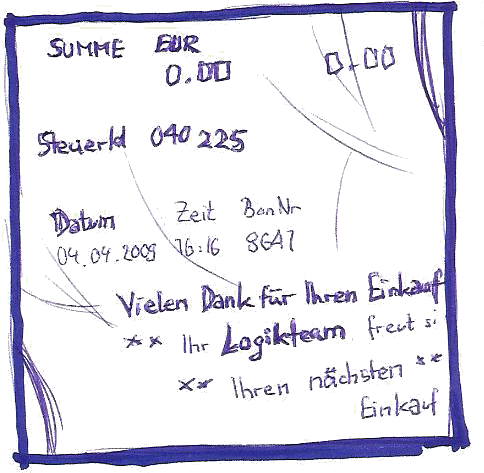
\includegraphics[scale=0.3]{evidence.png}};
  \end{tikzpicture}

  \note{
    \begin{definition}
      \begin{itemize}
        \item $\neg A \ :\equiv\ (A \Rightarrow \bot).$
        \item Einen Beleg für~$\bot$ gibt es nicht.
      \end{itemize}
    \end{definition}

    \tikz[remember picture] \node[coordinate,yshift=0.0em] (n0) {};
    \vspace{-1.5em}
    \begin{description}\small
      \item[$\neg A$] $A$ stimmt nicht.
      \tikz[remember picture] \node[coordinate,yshift=0.5em] (n2) {};
      \item[$\neg \neg A$] $A$ stimmt.
      \tikz[remember picture] \node[coordinate,yshift=-0.0em] (n1) {};
    \end{description}
    \vspace{1em}

    \begin{description}\small
      \item[$\neg A$] Es kann keinen Beleg für~$A$ geben.
      \tikz[remember picture] \node[coordinate,yshift=0.5em] (n5) {};%
      \item[$\neg \neg A$] Es kann keinen Beleg für~$\neg A$ geben
      (gewissermaßen ist $A$
      "`potenziell wahr"').
      \tikz[remember picture] \node[coordinate,yshift=-0.0em] (n4) {};
    \end{description}

    \begin{tikzpicture}[overlay,remember picture]
      \path (n2) -| node[coordinate] (n3) {} (n0);
      \path (n1) -| node[coordinate] (n33) {} (n0);
      \draw[thick,decorate,decoration={brace,amplitude=5pt}]
              (n33) -- (n3) node[midway,left=4pt] {kl.};
      \path (n5) -| node[coordinate] (n6) {} (n0);
      \path (n4) -| node[coordinate] (n44) {} (n0);
      \draw[thick,decorate,decoration={brace,amplitude=5pt}]
              (n44) -- (n6) node[midway,left=4pt] {int.};
    \end{tikzpicture}
  }
}

\subsection{Das Axiom vom ausgeschlossenen Dritten}
\frame[t]{\frametitle{Das Axiom vom ausgeschlossenen Dritten}
  \begin{axiom}[\emph{LEM}, klassisch]
    Für jede Aussage~$A$ kann man
    \[ A \,\vee\, \neg A \]
    ableiten.
  \end{axiom}

  \begin{itemize}
    \item Klassische Interpretation: \\ Eine jede Aussage stimmt oder stimmt nicht.
    \item Intuitionistische Interpretation: \\ Für jede Aussage haben wir jeweils Beleg
    für sie oder für ihre Negation.
    \vfill
    \item intuitionistische Logik $:=$
          klassische Logik ohne LEM
  \end{itemize}

  \begin{tikzpicture}[remember picture,overlay]  
    \node [xshift=-1.7cm,yshift=-3.8cm] at (current page.north east)
      {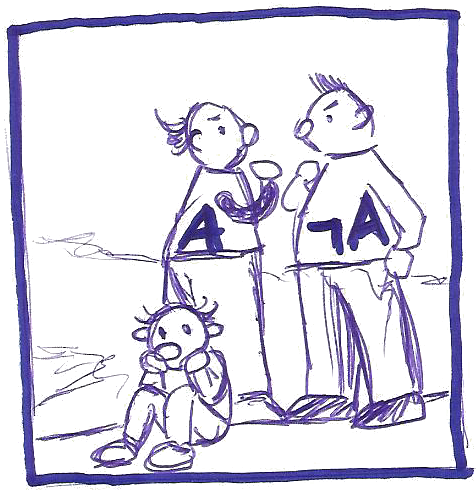
\includegraphics[scale=0.4]{lem.png}};
  \end{tikzpicture}
}

\note{
  \vspace{-1em}
  \begin{itemize}
    \item Die intuitionistische Interpretation von LEM ist offensichtlich
          falsch.
    \item Intuitionistische Logik ist abwärtskompatibel zu klassischer Logik:
          Alles, was intuitionistisch ableitbar ist, ist auch klassisch ableitbar.
          Insbesondere ist die Negation von LEM kein Axiom.
    \item Auch intuitionistisch gilt $\neg(A \wedge \neg A)$: Angenommen, wir
          hätten Beleg für $A \wedge \neg A$. Dann haben wir Beleg
          für~$A$ und können aus Belegen für~$A$ Belege für~$\bot$
          konstruieren. Also erhalten wir Beleg für~$\bot$.
  \end{itemize}
}

\note{
  \begin{proposition}
    Das Axiom vom ausgeschlossenen Dritten (LEM),
    \[ A \ \vee\ \neg A \]
    für alle Aussagen~$A$, ist äquivalent zum Axiom der
    Doppelnegationselimination (DNE),
    \[ \neg\neg A \ \Rightarrow\ A \]
    für alle Aussagen~$A$.
  \end{proposition}
  \begin{proof}
    Gelte LEM. Gelte~$\neg\neg A$. Dann gilt nach LEM $A$ oder~$\neg A$.
    Letzteres kann nicht eintreten, also folgt~$A$.

    Gelte umgekehrt DNE. Dann genügt es, $\neg\neg(A \vee \neg A)$ zu zeigen.
    Angenommen $\neg(A \vee \neg A)$. Dann folgt~$\neg A$ (wieso?) und analog
    $\neg\neg A$. Das ist ein Widerspruch.
  \end{proof}
}

\frame[t]{\frametitle{Irrational hoch irrational}
  \begin{definition}
    Eine reelle Zahl heißt genau dann \emph{irrational}, wenn sie
    nicht rational ist, d.\,h. wenn sie sich nicht als Bruch
    \[ \frac{a}{b} \]
    mit $a$, $b \in \mathbb{Z}$ schreiben lässt.
  \end{definition}

  \begin{theorem}
    Es gibt irrationale Zahlen~$x$, $y$, sodass $x^y$ rational ist.
  \end{theorem}

  \note{
    \begin{proof}[Beweis (klassisch, mit LEM)]
      Es ist~$\sqrt{2}^{\sqrt{2}}$ rational oder irrational. Setze im ersten
      Fall
      \begin{align*}
        x &:= \sqrt{2}, & y &:= \sqrt{2},
      \intertext{im zweiten}
        x &:= \sqrt{2}^{\sqrt{2}}, & y & := \sqrt{2}. \qedhere
      \end{align*}
    \end{proof}
  }

  \note{
    \begin{proof}[Beweis (intuitionistisch und klassisch zulässig)]
      Setze~$x := \sqrt{2}$, $y := \log_{\sqrt{2}} 3$. Dann $x^y = 3$.
    \end{proof}
  }
}

\subsection{Anwendungen}
\frame[t]{\frametitle{Anwendungen}
  \only<1>{
    \begin{center}
      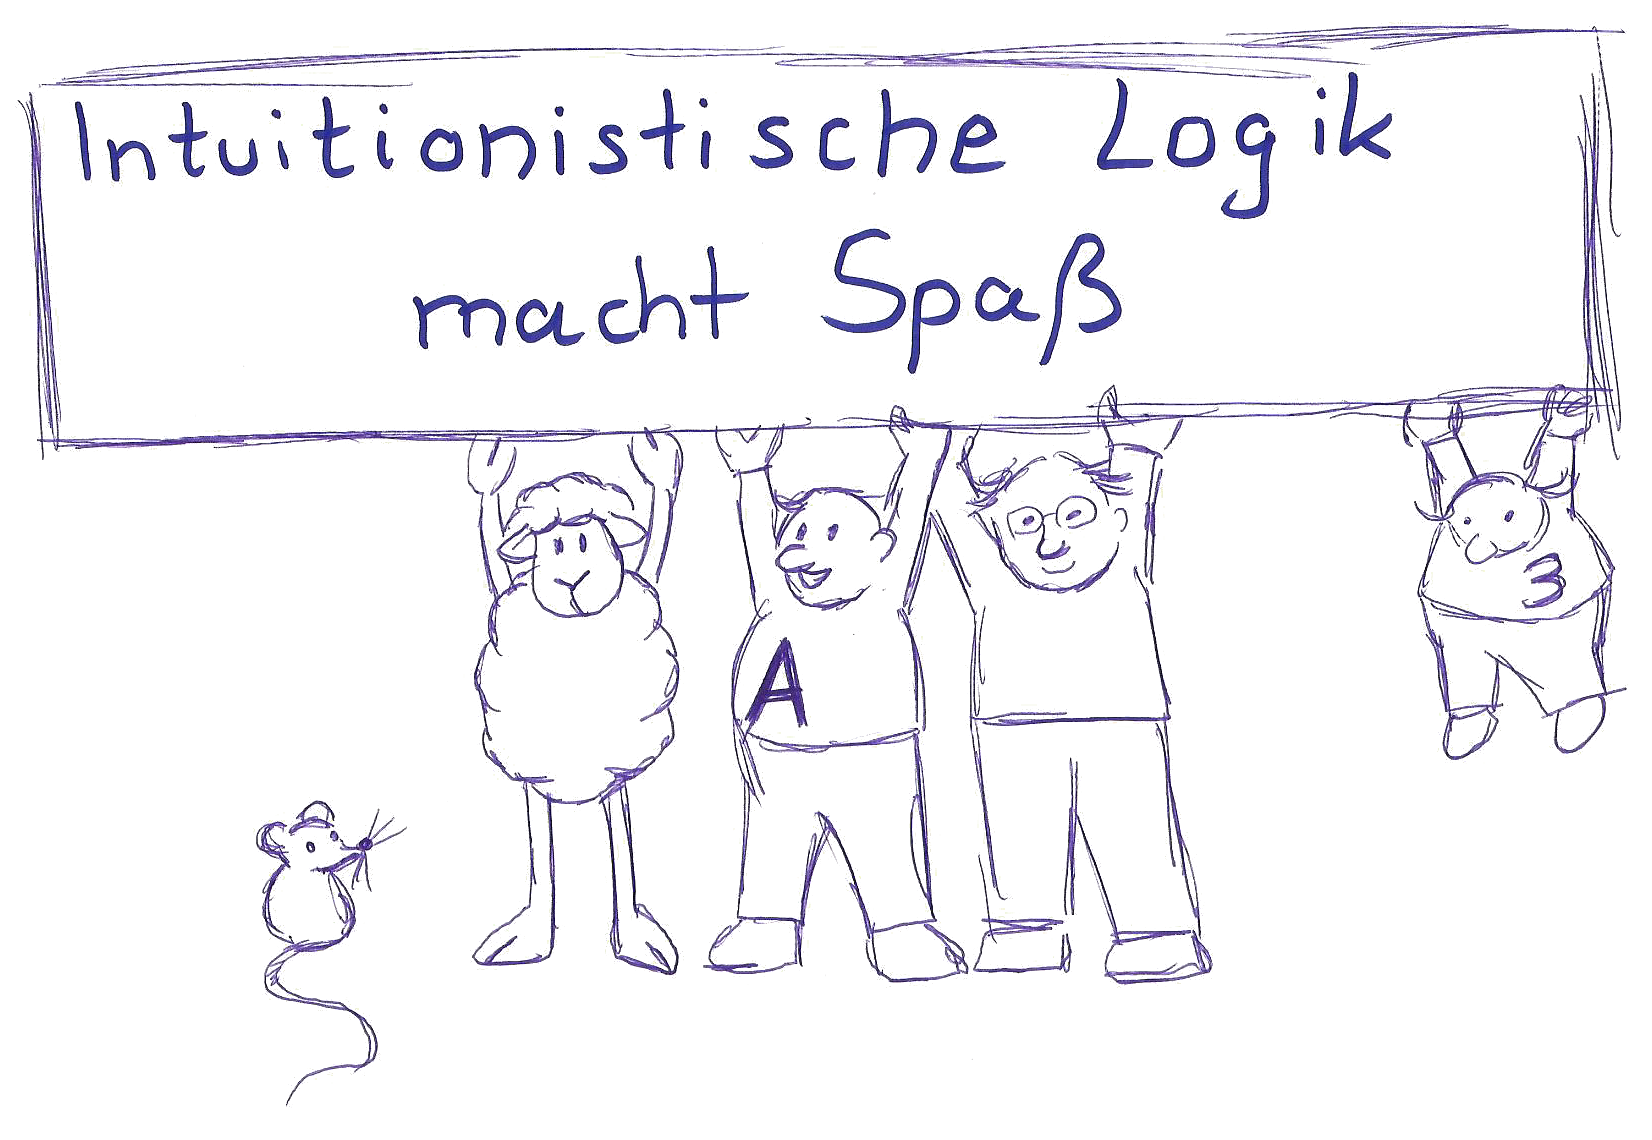
\includegraphics[scale=0.4]{fun.png}
    \end{center}
  }
  \pause

  \begin{itemize}
    \item Mit intuitionistischer Logik kann man Belegbarkeitsfragen untersuchen.
    \item Aus intuitionistischen Beweisen kann man maschinell \emph{Programme} extrahieren.
    \item Die \emph{interne Sprache} von Topoi ist i.\,A. intuitionistisch.
    \item Intuitionistisch kann man \emph{Traummathematik} studieren.
  \end{itemize}

  \vfill
  \begin{center}
    \phantom{a}
    \hfill
    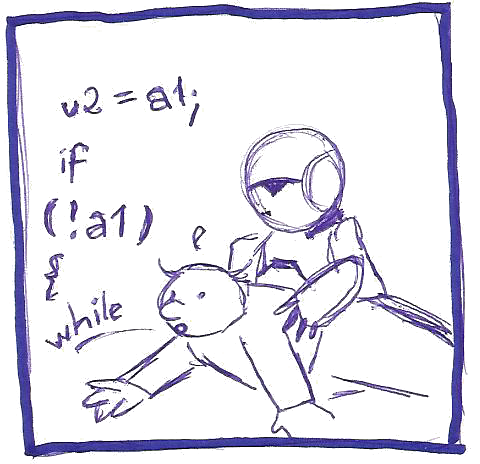
\includegraphics[scale=0.4]{program-extraction.png}
    \hfill
    
\includegraphics[scale=0.4]{constructive-maths.png}
    \hfill
    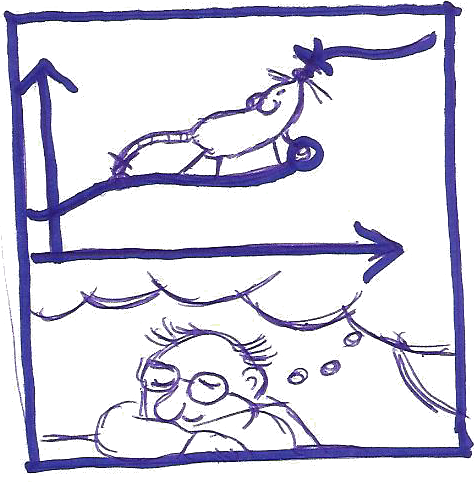
\includegraphics[scale=0.4]{dream-maths.png}
    \hfill
    \phantom{a}
  \end{center}

  \note<2>{
    \begin{itemize}
      \item Intuitionistische Logik formalisiert (eine Spielart der)
            konstruktiven Mathematik.
      \item Sehr viele Teilgebiete der Mathematik (auch analytische)
            lassen sich intuitionistisch behandeln. Dabei muss man manchmal
            Zusatzvoraussetzungen fordern, die klassisch stets erfüllt sind.
            Üblicherweise empfindet man das nicht als Nachteil, sondern als
            willkommenes Mittel, um abstrakte Konzepte und Zusammenhänge besser zu
            verstehen.
      \item Beispiele für Traumaxiome sind:
            \begin{itemize}
              \item \emph{Alle Funktionen sind stetig.}
              \item \emph{Es gibt nilquadratische Zahlen~$x$ (d.\,h. Zahlen mit $x^2 = 0$),
            die aber selbst nicht null sind.}
            \end{itemize}
            Diese führen klassisch sofort
            zu einem Widerspruch, intuitionistisch aber nicht.
    \end{itemize}
  }
}

\section{Eine andere mathematische Welt}

\subsection{Leere und nichtleere Mengen}
\frame[t]{\frametitle{Leere und nichtleere Mengen}
  Sei~$X$ eine Menge.
  
  \emph{Frage:} Sind die beiden folgenden Aussagen
  äquivalent?
  \begin{enumerate}
    \item $X$ ist \emph{nicht leer}, d.\,h. $X \neq \emptyset$.
    \item $X$ ist \emph{bewohnt}, d.\,h. $\exists x \in X$.
  \end{enumerate}

  \visible<2>{
  Aussage~{\insertenumlabel} ist stärker: Wir können explizit ein Element~$x$ der
  Menge angeben.
  }

  \vfill
  \begin{center}
    
\includegraphics[scale=0.4]{empty-set.png}
    \hfill
    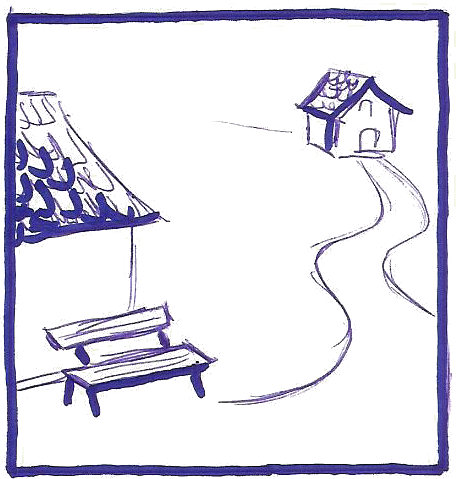
\includegraphics[scale=0.4]{schwebe-set.png}
    \hfill
    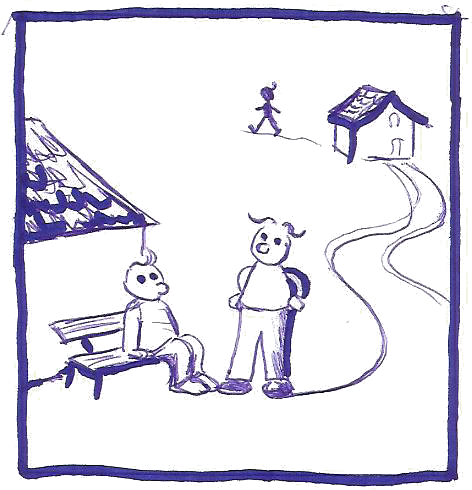
\includegraphics[scale=0.4]{inhabited-set.png}
  \end{center}

  \note<2>{
    \begin{proposition}
      Wenn für alle Mengen~$X$ aus Nichtleerheit schon Bewohntheit folgt, gilt
      DNE (und damit LEM).
    \end{proposition}
    \begin{proof}
      Sei~$A$ eine Aussage und gelte~$\neg\neg A$. Definiere $X := \{ \star \,|\, A \}$. Dann gilt~$X
      \neq \emptyset$, denn das ist gleichbedeutend mit~$\neg\neg \exists x
      \in X$, also mit~$\neg \neg A$. Nach Voraussetzung folgt damit~$\exists x \in
      X$, also~$A$.
    \end{proof}
  }
}

\subsection{Teilmengen der Eins}
\frame[t]{\frametitle{Teilmengen der Eins}
  \begin{definition}Die \emph{Menge der Wahrheitswerte~$\Omega$} ist
  die Menge aller Teilmengen der Menge
  \[ \1 := \{ \star \}, \]
  also
  \[ \Omega := \P(\1) = \{ U \,|\, U \subseteq \1 \}. \]
  \end{definition}

  \begin{itemize}
    \item \emph{Frage:} Wie viele Elemente enthält~$\Omega$?
    \pause
    \item Es gibt auch
    \begin{align*}
      \Omega_{\text{entscheidbar}} &:= \{ p \in \Omega \,|\, \star \in p \ \vee\ 
      \star \not\in p \}, \\
      \Omega_{\text{stabil}} &:= \{ p \in \Omega \,|\, \neg \neg(\star \in
      p) \ \Rightarrow\  \star \in p \}.
    \end{align*}
    In welcher Beziehung stehen diese zu~$\Omega$?
  \end{itemize}

  \note<2>{
    \vspace{-1em}
    \begin{scriptsize}\begin{itemize}
      \item Klassisch gilt~$\Omega = \{ \emptyset, \{ \star \} \}$, aber
            intuitionistisch kann man nur~"`$\supseteq$"' zeigen.
      \item \vspace{-0.5em} Sind~$A$ und~$B$ Aussagen, hat man beispielsweise zumindest
            folgende Elemente von~$\Omega$ (und noch viele weitere):
            \vspace{-0.5em}
            \begin{center}\begin{tikzpicture}[node distance=0.7cm]
              \node (T)                {$\{ \star \}$};
              \node (P)  [below of=T]  {};
              \node (A)  [left  of=P]  {$\{ \star \,|\, A \}$};
              \node (B)  [right of=P]  {$\{ \star \,|\, B \}$};
              \node (AB) [below of=P]  {$\{ \star \,|\, A \wedge B \}$};
              \node (F)  [below of=AB] {$\emptyset$};
              \draw (T)  -- (A);
              \draw (T)  -- (B);
              \draw (A)  -- (AB);
              \draw (B)  -- (AB);
              \draw (AB) -- (F);
            \end{tikzpicture}\end{center}
      \item \vspace{-0.5em} Man kann aber nicht zeigen, dass diese Zwischenmengen
      ungleich~$\{ \star \}$ und ungleich~$\emptyset$ sind
      (Abwärtskompatibilität zur klassischen Logik!).
      \item \vspace{-0.5em} Es gilt $\Omega_{\text{entscheidbar}} = \{ \emptyset, \{ \star \} \}$ und
            $\Omega_{\text{entscheidbar}} \subseteq \Omega_{\text{stabil}} \subseteq \Omega$.
      \item \vspace{-0.5em} Die Bezeichung \emph{entscheidbar} hat eine anschauliche
            Interpretation in der Informatik: Entscheidbare Aussagen sind
            solche, für die wir einen Algorithmus angeben können, der (in
            endlicher Zeit) prüft, ob die Aussage gilt oder nicht.
    \end{itemize}\end{scriptsize}
  }
}

\subsection{Minima von Mengen natürlicher Zahlen}
\frame[t]{\frametitle{Minima von Mengen natürlicher Zahlen}
  Klassisch gilt: Jede bewohnte Menge natürlicher Zahlen besitzt ein Minimum.

  \emph{Frage:} Stimmt das auch intuitionistisch?

  \vspace{1em}
  \begin{center}
    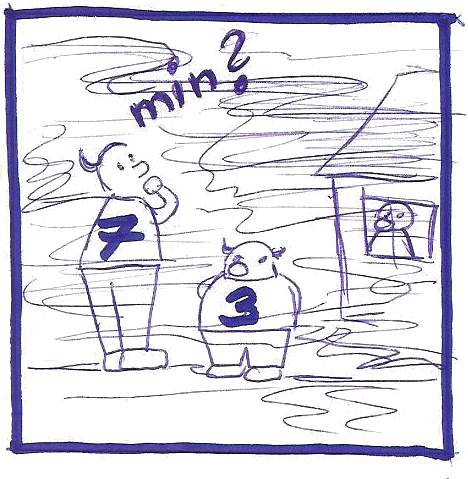
\includegraphics[scale=0.6]{minima.png}
  \end{center}

  \note{
    \begin{proposition}
      Wenn alle bewohnten Mengen natürlicher Zahlen ein Minimum besitzen, gilt
      LEM.
    \end{proposition}
    \begin{proof}
      Sei~$A$ eine Aussage. Wir definieren die Menge
      \[ X := \{ 1 \} \cup \{ 0 \,|\, A \} \subseteq \mathbb{N}. \]
      Dann ist~$X$ bewohnt (da~$1 \in X$) und besitzt daher nach Voraussetzung
      ein Minimum~$x \in \mathbb{N}$.
      Es ist~$\mathbb{N}$ diskret, daher folgt~$x = 0$ oder~$x \neq 0$. Im
      ersten Fall folgt~$A$, im zweiten~$\neg A$.
    \end{proof}

    Man kann mit einer Zusatzvoraussetzung das Prinzip retten: Alle
    bewohnten und herauslösbaren Teilmengen $X \subseteq \mathbb{N}$ (d.\,h.
    solche mit
    $\forall x \in \mathbb{N}\_ x \in X \vee x \not\in X$) besitzen ein
    Minimum.
  }
}

\subsection{Endliche Mengen}
\frame[t]{\frametitle{Endliche Mengen}
  \begin{definition}
    Sei~$X$ eine Menge. $X$ heißt\ldots
    \begin{itemize}
      \item \ldots\emph{endlich} \tabto{3.4cm} $:\Leftrightarrow$
        $\exists n \in \N\_ \exists f{:}\, [n] \to X\_ \text{$f$ bijektiv}$.
      \item \ldots\emph{endlich indiziert} \tabto{3.4cm} $:\Leftrightarrow$
        $\exists n \in \N\_ \exists f{:}\, [n] \to X\_ \text{$f$ surjektiv}$.
    \end{itemize}
    Dabei ist~$[n] := \{ m \in \N \,|\, m < n \} = \{ 0, 1, \ldots, n-1 \}$.
  \end{definition}

  \emph{Frage:} \tabto{1.2cm} Sind Teilmengen endlicher (endl. indizierter) \\
  \tabto{1.2cm} Mengen wieder endlich (endl. indiziert)?

  \begin{tikzpicture}[remember picture,overlay]  
    \node [xshift=-2.0cm,yshift=-7.8cm] at (current page.north east)
      {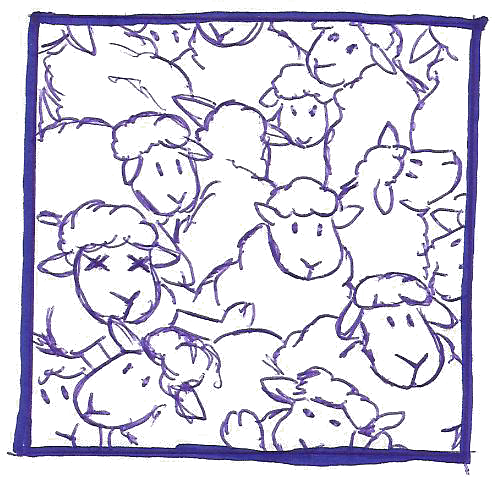
\includegraphics[scale=0.4]{many-sheep.png}};
  \end{tikzpicture}

  \note{\begin{itemize}
    \item Die Mengen~$[n]$ für~$n \in \mathbb{N}$ stellen wir uns
          als die Prototypen endlicher Mengen vor.
    \item Aus \emph{endlich} folgt \emph{endlich indiziert}.
          Die Umkehrung gilt für diskrete Mengen.
    \item Endlich indizierte Mengen sind entweder leer oder bewohnt.
          (Bei beliebigen Mengen kann man diese Disjunktion nicht zeigen.)
    \item Sollten Teilmengen endlich indizierter Mengen stets wieder
          endlich indiziert sein, gilt LEM. Um das zu zeigen, betrachtet man geeignete
          Teilmengen der endlich indizierten (sogar endlichen) Menge~$\1 =
          \{\star\}$.
    \item Es gibt noch weitere Endlichkeitsbegriffe, die für manche
          Anwendungen besser oder schlechter geeignet sind.
  \end{itemize}}
}


\section{Eleganzassistenz}

\subsection{Unendlichkeit der Primzahlen}
\frame[t]{\frametitle{Unendlichkeit der Primzahlen}
  \begin{theorem}[schwache Form]Die Menge~$\mathbb{P}$ der Primzahlen,
  \[ \mathbb{P} := \{ 2, 3, 5, 7, 11, 13, \ldots \} \subseteq \N, \]
  ist nicht endlich.\end{theorem}
  \pause

  \begin{theorem}[starke Form]Sei~$S$ eine endliche Menge von Primzahlen. Dann gibt es
  eine weitere Primzahl, die nicht in~$S$ enthalten ist.\end{theorem}

  \note<2>{\begin{itemize}
    \item Die schwache Formulierung hat wegen der negativen Behauptung keinen
    algorithmischen Inhalt.
    \item Aus einem intuitionistischen Beweis der starken Form kann man
    maschinell einen entsprechenden Algorithmus extrahieren.
    \item Euklids Beweis der starken Form ist kürzer und klarer als der der
    schwachen Form, und zeigt auch noch eine stärkere Aussage.
    \item Empirisches Faktum: Versucht man, klassische Theorien
    intuitionistisch zu entwickeln, stößt man auf einfachere und elegantere
    Konzepte und Beweise.
  \end{itemize}}
}

\subsection{Übungsaufgabe in Linearer Algebra I}
\frame[t]{\frametitle{Übungsaufgabe in Linearer Algebra I}
  \begin{proposition}
    Sei~$f{:}\, X \to Y$ eine Abbildung und sei
    \[ \renewcommand{\arraystretch}{1.3}\begin{array}{@{}rrcl@{}}
      \varphi{:} &\P(Y)&\longrightarrow& \P(X), \\
      & U &\longmapsto& f^{-1}[U] := \{ x \in X \,|\, f(x) \in U \}
    \end{array} \]
    die zugehörige Urbildoperation. Dann ist~$f$ genau dann surjektiv,
    wenn~$\varphi$ injektiv ist.
  \end{proposition}

  \emph{Zum Knobeln:} Auch für die Rückrichtung gibt es einen direkten Beweis.

  \note{
    \begin{proof}[Beweis (umständlich, nur klassisch zulässig)]
      Angenommen,~$f$ ist nicht surjektiv. Dann gibt es ein~$y \in Y$, welches
      nicht im Bild von~$f$ liegt. Somit gilt~$\varphi(\{y\}) = \emptyset =
      \varphi(\emptyset)$ im Widerspruch zur Injektivität von~$\varphi$.
    \end{proof}
    \rotatebox{180}{\vbox{
    \begin{proof}[Beweis (elegant)]
      Es gilt~$\varphi(\Bild f) = X = \varphi(Y)$, also~$\Bild f = Y$.
    \end{proof}}}
  }
}

\section{Gentzens Kalkül natürlichen Schließens}
\frame[t]{\frametitle{Gentzens Kalkül natürlichen Schließens}
  \small
  \begin{itemize}
    \item Strukturelle Regeln: \\
    \vspace{-1em}
    \phantom{a}\hfill
    \AxiomC{$\phantom{\seq{\vec x}}$}\UnaryInfC{$A \seq{\vec x} A$}\DisplayProof\hfill
    \AxiomC{$A \seq{\vec x} B$}\UnaryInfC{$A[\vec s/\vec x]
    \seq{\vec y} B[\vec s/\vec x]$}\DisplayProof\hfill
    \AxiomC{$A \seq{\vec x} B$}\AxiomC{$B \seq{\vec x}
    C$}\BinaryInfC{$A \seq{\vec x} C$}\DisplayProof\hfill
    \phantom{a}
    \vspace{-0.3em}
    \item Regeln für Konjunktion: \\
    \AxiomC{$\phantom{\seq{\vec x}}$}\UnaryInfC{$A \seq{\vec x} \top$}\DisplayProof\hfill
    \AxiomC{$\phantom{\seq{\vec x}}$}\UnaryInfC{$A \wedge B \seq{\vec x} A$}\DisplayProof\hfill
    \AxiomC{$\phantom{\seq{\vec x}}$}\UnaryInfC{$A \wedge B \seq{\vec x} B$}\DisplayProof\hfill
    \AxiomC{$A \seq{\vec x} B$}\AxiomC{$A \seq{\vec x} C$}\BinaryInfC{$A \seq{\vec x} B \wedge C$}\DisplayProof
    \vspace{-0.3em}
    \item Regeln für Disjunktion: \\
    \AxiomC{$\phantom{\seq{\vec x}}$}\UnaryInfC{$\bot \seq{\vec x} A$}\DisplayProof\hfill
    \AxiomC{$\phantom{\seq{\vec x}}$}\UnaryInfC{$A \seq{\vec x} A \vee B$}\DisplayProof\hfill
    \AxiomC{$\phantom{\seq{\vec x}}$}\UnaryInfC{$B \seq{\vec x} A \vee B$}\DisplayProof\hfill
    \AxiomC{$A \seq{\vec x} C$}\AxiomC{$B \seq{\vec x} C$}\BinaryInfC{$A \vee B \seq{\vec x} C$}\DisplayProof
    \vspace{-0.3em}
    \item Doppelregel für Implikation: \\
    {\centering \AxiomC{$A \wedge B \seq{\vec x} C$}\doubleLine\UnaryInfC{$A \seq{\vec x} B \Rightarrow C$}\DisplayProof\par}
    \vspace{-0.3em}
    \item Doppelregeln für Quantifikation: \\
    \vspace{-0.7em}
    \phantom{a}\hfill
    \AxiomC{$A \seq{\vec x, y} B$}\doubleLine\UnaryInfC{$\exists y\_\! A \seq{\vec x} B$}\DisplayProof\hfill
    \AxiomC{$A \seq{\vec x, y} B$}\doubleLine\UnaryInfC{$A \seq{\vec x} \forall y\_\! B$}\DisplayProof\hfill
    \phantom{a}
  \end{itemize}

  \note{
    \begin{itemize}
      \item Vorkommende Variablen sind in der Notation unterdrückt.
      \item Exemplarisch bedeutet die Regel für Implikation folgendes:
            Genau dann, wenn sich unter der Annahme~$A \wedge B$ die Formel~$C$
            herleiten lässt, lässt sich auch unter der Annahme von~$A$ die
            Formel~$(B \Rightarrow C)$ herleiten.
      \item Unter der anfangs gegebenen informalen Bedeutung sind all diese Regeln plausibel.
      \item Die Regeln für Disjunktion und Konjunktion sind zueinander dual.
      \item Das Axiom vom ausgeschlossenen Dritten sieht in der Regelschreibweise so aus: \\
            {\centering \AxiomC{$\phantom{\seq{\vec x}}$}\UnaryInfC{$\seq{\vec x} A \vee \neg A$}\DisplayProof\par}
    \end{itemize}
  }
}

\note{
  \begin{itemize}
    \item Die Regel für den Existenzquantor muss auf solche Formeln~$B$ eingeschränkt werden, in denen die Variable~$y$
          nicht vorkommt. Analog darf bei der Regel für den Allquantor in der Formel~$A$ kein~$y$ vorkommen.
    \item Die Regel für den Existenzquantor rechtfertigt folgendes informelles Beweisschema, um
          aus der Annahme~$\exists y\_\! A$ eine Formel~$B$ zu folgern:

          \emph{Gelte $\exists y\_\! A$. Dann gibt es ein~$y$ mit~$A$. \dots Also gilt~$B$.}
    \item Analog rechtfertigt die Regel für den Allquantor folgendes Vorgehen,
          um aus der Annahme~$A$ die Formel~$\forall\! y\_ B$ abzuleiten:

          \emph{Gelte~$A$. Sei~$y$ beliebig. \dots Also gilt~$B$.}
  \end{itemize}
}

\section{Semantik}

\subsection{Heytingmodelle}
\frame[t]{\frametitle{Heytingalgebren}
  \begin{definition}
    Eine \emph{Heytingalgebra}~$H$ ist eine partiell geordnete Menge~($\leq$), in der
    \begin{enumerate}
    \item alle endlichen Infima~($\sqcap$) und Suprema~($\sqcup$) existieren,
    \item zu je zwei Elementen~$a,b \in H$ ein Element $(a \to b) \in H$ mit
    \[ x \sqcap a \leq b \quad\text{gdw.}\quad x \leq (a \to b) \]
    für alle~$x \in H$ existiert.
    \end{enumerate}
  \end{definition}

  \vfill
  \begin{itemize}
    \item Beispiele für Heytingalgebren: $\{ 0, \nicefrac{1}{2}, 1\}$, $\P(\1)$, $\O(X)$
    \item Wir stellen uns Elemente einer Heytingalgebra als (verallgemeinerte)
    Wahrheitswerte vor.
  \end{itemize}

  \note{
    \begin{itemize}
      \item Die definierende universelle Eigenschaft von~$({\to})$ ist genau so
      gemacht, dass sie der Schlussregel für die Implikation im Gentzenkalkül
      entspricht.
      \item Für ein Element~$a \in H$ ist~$(a \to \bot)$ das sog.
      \emph{Pseudokomplement} von~$a$. Im Allgemeinen gilt natürlich nicht $a
      \sqcup (a \to \bot) = \top$.
    \end{itemize}
  }
}

\frame[t]{\frametitle{Heytingmodelle I\phantom{I}}
  \begin{definition}
    Ein \emph{Heytingmodell} besteht aus
    \begin{enumerate}
      \item einer Heytingalgebra~$H$ und
      \item einer Zuordnung~$\ll{\cdot}$ von Formeln zu Elementen aus~$H$
    \end{enumerate}
    sodass die Axiome
    \begin{align*}
      \ll{\top} &= \text{größtes Element von~$H$} \\
      \ll{\bot} &= \text{kleinstes Element von~$H$} \\
      \ll{A \wedge B} &= \ll{A} \sqcap \ll{B} \\
      \ll{A \vee B} &= \ll{A} \sqcup \ll{B} \\
      \ll{A \Rightarrow B} &= \ll{A} \to \ll{B}
    \end{align*}
    für alle Formeln~$A$, $B$ erfüllt sind.
  \end{definition}
}

\frame[t]{\frametitle{Heytingmodelle II}
  \begin{theorem}
    \begin{enumerate}
      \item Heytingmodelle sind korrekt: Es gilt
            \[ A \seq{} B \quad\Rightarrow\quad \ll{A} \leq \ll{B} \]
            für alle Formeln $A$, $B$ und Heytingmodelle~$\ll{\cdot}$.
      \item Heytingmodelle sind auch vollständig: Gilt für gegebene Formeln $A$,
            $B$, dass
            \[ \ll{A} \leq \ll{B} \]
            für alle Heytingmodelle~$\ll{\cdot}$, so folgt $A \seq{} B$.
    \end{enumerate}
  \end{theorem}

  \note{
    \begin{proof}
      \begin{enumerate}
        \item Induktion über den Aufbau intuitionistischer Ableitungen im
        Gentzenkalkül.
        \item Die \emph{Lindenbaumalgebra}
              \[ L := (\text{Menge aller Formeln})/(\text{ableitbare Äquivalenz}) \]
              mit~$\ll{A} := [A]$ (Äquivalenzklasse von~$A$) ist ein spezielles
              Heytingmodell, in dem $[A] \leq [B]$ gleichbedeutend mit $A \seq{} B$ ist.
              \qedhere
      \end{enumerate}
    \end{proof}

    Das Konzept des Heytingmodells lässt sich von propositionaler
    Logik auf Prädikatenlogik erster und höherer
    Ordnung verallgemeinern; dann benötigt man nicht nur eine Heytingalgebra,
    sondern für jeden Typ der Sprache jeweils eine. Diese Daten organisieren
    sich zu einem Topos.
  }
}

\subsection{Kripkemodelle}
\frame[t]{\frametitle{Kripkemodelle}
  \begin{definition}
    Ein \emph{Kripkemodell} besteht aus
    \begin{enumerate}
      \item einer partiell geordneten Menge~$W$ von Welten und
      \item einer Erfüllbarkeitsrelation~$\models$
    \end{enumerate}
    sodass folgende Axiome erfüllt sind:
    \begin{enumerate}
      \item Aus $w \leq u$ und $w \models A$ folgt $u \models A$.
      \item $w \models \bot$ stimmt nicht.
      \item $w \models A \wedge B$ \tabto{2.3cm} gdw. $w \models A$ und $w \models B$.
      \item $w \models A \vee B$ \tabto{2.3cm} gdw. $w \models A$ oder $w \models B$.
      \item $w \models A \Rightarrow B$ \tabto{2.3cm} gdw. für alle~$u$ mit~$w
      \leq u$: \\ \tabto{2.3cm} ${\qquad}$ Aus $u \models A$ folgt $u \models B$.
    \end{enumerate}
  \end{definition}

  \note{\begin{itemize}
    \item $w \models \neg A$ gdw. $\neg\exists v \geq w\_ v \models A$.
    \item $w \models \neg\neg A$ gdw. $\forall v \geq w\_ \neg\neg\exists u
    \geq v\_ u \models A$.
  \end{itemize}}
}

\section{Doppelnegationsübersetzung}
\frame[t]{\frametitle{Doppelnegationsübersetzung I\phantom{II}}
  \begin{definition}
    \begin{itemize}
      \item
        Eine Aussage~$A$ heißt genau dann \emph{entscheidbar}, wenn
        \[ A \ \vee\  \neg A. \]
      \item
        Eine Aussage~$A$ heißt genau dann \emph{stabil}, wenn
        \[ \neg\neg A \ \Rightarrow\  A. \]
    \end{itemize}
  \end{definition}

  \vfill
  Beispiele:
  \begin{itemize}
    \item "`$n = m$"' ist für natürliche Zahlen $n$, $m$ entscheidbar.
    \item Entscheidbare Aussagen sind auch stabil.
    \item Jede Aussage der Form $\neg\neg B$ ist stabil.
  \end{itemize}

  \note{
    \begin{proof}
      \begin{enumerate}
        \item Das folgt mit Induktion.
        \item Folgt wie beim Beweis LEM\,$\Rightarrow$\,DNE.
        \item Allgemein gilt~$\neg\neg\neg A \Rightarrow \neg A$: Denn
        angenommen~$A$. Dann folgt~$\neg\neg A$ (wieso?). Da aber~$\neg\neg\neg A$,
        folgt~$\bot$. \qedhere
      \end{enumerate}
    \end{proof}
  }
}

\frame[t]{\frametitle{Doppelnegationsübersetzung II\phantom{I}}
  \begin{definition}
    Die Doppelnegationsübersetzung~$A^\circ$ ist für Aussagen~$A$ wie folgt
    rekursiv definiert:
    \begin{align*}
      A^\circ &:= \neg\neg A \text{ für atomare Aussagen~$A$} \\
      (A \wedge B)^\circ &:= A^\circ \wedge B^\circ \\
      (A \vee B)^\circ &:= \neg(\neg A^\circ \wedge \neg B^\circ) \\
      (A \Rightarrow B)^\circ &:= A^\circ \Rightarrow B^\circ \\
      (\forall x\?X\_ A(x))^\circ &:= \forall x\?X\_ A^\circ(x) \\
      (\exists x\?X\_ A(x))^\circ &:= \neg\forall x\?X\_ \neg A^\circ(x)
    \end{align*}
  \end{definition}
}

\frame[t]{\frametitle{Doppelnegationsübersetzung III}
  \begin{theorem}
    \begin{enumerate}
      \item Klassisch gilt $A \Leftrightarrow A^\circ$ für alle Aussagen~$A$.
      \item Intuitionistisch sind alle Aussagen der Form~$A^\circ$ stabil.
      \item Wenn für alle betrachteten atomaren Aussagen~$A$ gilt, dass
            aus der klassischen Ableitbarkeit von~$A$ die intuitionistische
            Ableitbarkeit von $A^\circ$ folgt, so gilt das auch für alle
            zusammengesetzten Aussagen.
    \end{enumerate}
  \end{theorem}

  \begin{corollary}
    Peanoarithmetik (d.\,h. das System der fünf Peanoaxiome in klassischer Logik)
    ist genau dann konsistent, wenn Hey\-ting\-arith\-me\-tik (dieselben Axiome
    in intuitionistischer Logik) es ist.
  \end{corollary}

  \note{
    \begin{proof}[Beweis des Satzes]
      \begin{enumerate}
        \item Klar (Induktion über den Formelaufbau).
        \item Einfach (Induktion über den Formelaufbau).
        \item Einfach (noethersche Induktion über den Aufbau klassischer
        Ableitungen im Gentzenkalkül unter Verwendung der gezeigten Stabilität). \qedhere
      \end{enumerate}
    \end{proof}

    \begin{proof}[Beweis des Korollars]
      Zeigt Peanoarithmetik einen Widerspruch, so zeigt Heytingarithmetik
      $\bot^\circ$. Das ist äquivalent zu $\bot$.
    \end{proof}
  }
}

\note{
  \small
  Weitere wichtige Stichpunkte:

  \begin{itemize}
    \item \emph{Satz von Barr:} Aussagen einer gewissen syntaktischen Form (sog. \emph{geometrische
    Aussagen}, aber die Bezeichnung ist zunächst irreführend) lassen sich genau
    dann klassisch ableiten, wenn sie sich intuitionistisch ableiten lassen.
    Dieses Metatheorem kann man allerdings nur mit klassischer Logik zeigen.

    \item \emph{Curry-Howard-Korrespondenz:} Logische Formeln entsprechen
    Typen, Beweise der Formeln Termen dieser Typen. Unter dieser Korrespondenz
    geht die Doppelnegationsübersetzung in die
    \emph{Continuation Passing Transformation} (CPS) über.

    \item Eine Formalisierung konstruktiver Mengenlehre ist
    \emph{Intuitionistic Zermelo Fraenkel} (IZF). In ihr ist das
    Auswahlaxiom nicht enthalten, da aus ihm der Satz vom ausgeschlossenen
    Dritten folgt (und da es unter den üblichen Interpretationen auch
    offensichtlich falsch ist).
  \end{itemize}
}

\section*{Literaturhinweise}
\frame[t]{\frametitle{Literaturhinweise}
  \scriptsize
  \begin{itemize}
    \item Beispiele für konstruktive Mathematik: \\
          \href{http://math.andrej.com/category/constructive-math/}{A. Bauer.
          Blog auf \texttt{http://math.andrej.com/}.} \\
          \href{http://alg.math.uni-augsburg.de/lehre/vorlesungsskripte/linalg.pdf/at_download/file}{M. Nieper-Wißkirchen.
          Lineare Algebra I und II. Vorlesungsskript, 2008.} \\
          \href{http://alg.math.uni-augsburg.de/lehre/vorlesungsskripte/einfuhrung-in-die-algebra/at_download/file}{M. Nieper-Wißkirchen. 
          Galoissche Theorie. Unveröffentlicht, 2012.}
    \item Philosophische Einordnung: \\
          \href{http://plato.stanford.edu/entries/logic-intuitionistic/}{J.
          Moschovakis. \emph{Intuitionistic Logic.} The Stanford Encyclopedia of
          Philosophy, 2010.}
    \item Beispiel für Traummathematik: \\
          A. Kock. \emph{Synthetic Differential Geometry.} Cambridge University
          Press, 2006.
    \item Einführungen in Topostheorie: \\
          S. Mac Lane, I. Moerdijk. \emph{Sheaves in Geometry and Logic: A First
          Introduction to Topos Theory.} Springer, 1992. \\
          P. Johnstone. \emph{Sketches of an Elephant: A Topos Theory
          Compendium.}
          Oxford University Press, 2002.
  \end{itemize}
}

\end{document}
